\documentclass[a4paper]{article}
\usepackage{graphicx} %Required for diagrams
\usepackage[bookmarks=true]{hyperref}
\usepackage{bookmark}%Required to do pdf bookmarking
\usepackage[margin=1.2in]{geometry}
\usepackage{float}
\usepackage{caption}
\usepackage{hyperref}%Required for referencing website pages
\usepackage[english]{babel}
%\usepackage[utf8x]{inputenc}
\usepackage{graphicx}
%\usepackage[colorinlistoftodos]{todonotes}

\title{Plan for Software Aspects of Certification}
\author{Baobab Team}

\begin{document}
\newpage

\input{./TitlePage.tex}
\newpage

\begin{center}
\textbf{\LARGE Member details\\}
\begin{tabular}{lr}
\\
Ephiphania Munava&10624610\\
Lutfiyya Razak&10198408\\
Lerato Molokomme&11197961\\
Mpedi Mello&11210754\\
Patience Mtsweni&11116774\\
Tsepo Ntsaba&10668544\\
\end{tabular}

\vspace{3cm}
\textbf{\LARGE Git repository link:\\}
\url{https://github.com/Ephiphania/Baobab}
\end{center}

\newpage

\tableofcontents
\listoffigures
\newpage
\setlength{\voffset}{-1cm}

\begin{center}
\begin{figure}
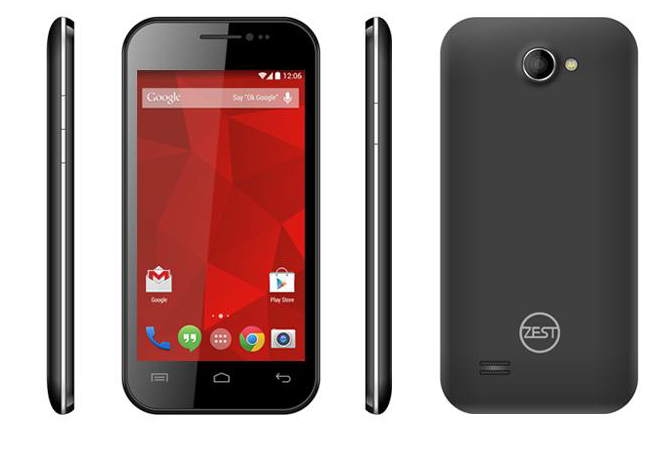
\includegraphics[width=1\linewidth]{./pictures/linphone.jpeg}
\caption{\label{fig:Linphone}3 of our members have been provided with a Zest T1 Android phone.}
\end{figure}
\end{center}

\newpage

%--------------------FunReq Create---------------------------s

\section{Introduction}

\subsection{Purpose}
\textbf{Description:}The purpose of this project is to extend Linphone's Instant Messaging (IM) implementation on Android platforms to include group chat and to implement other minor improvements to Linphones IM capabilities and user interface.
This project will give the student group exposure to:   
 \begin{itemize}
	\item Android development (Java and C)
	\item Open source contribution
	\item Cryptography
	\item Session initiation protocol (SIP)
	\item DO-178 certification
\end{itemize}
This project also forms part of a larger Masters study on development methodologies for projects seeking DO-178 certification.

\subsection{Scope}
\textbf{Description:}We are required to develop the following functionality for the Linphone project   
 \begin{itemize}
	\item Group chat (Invite additional members to a chat, all members receive chats)
	\item Secure group chat (AES256)
		\begin{itemize}
			\item A basic message encryption implementation will be provided
		\end{itemize}		 
	\item Creation and deletion of groups
	\item Voice record and send over IM
	\item Rework the messaging user interface
		\begin{itemize}
			\item Spacing between words are terrible
			\item Make the text bigger
			\item Block indents required to better specify who said what
			\item Presence indication to show a remote user is typing
			\item User picture portraits
		\end{itemize}		
\end{itemize}
\newpage

\section{Documentation conventions}
\textbf{Description:}DO-178B does not specify the documentation standard to be followed, but most projects do follow some or other documentation standard. The following figure is loosely based on MIL-STD-490A, although sometimes Detail design and Notes are changed into some other topic of discussion.\\

\begin{center}
\begin{figure}[h]
\centering
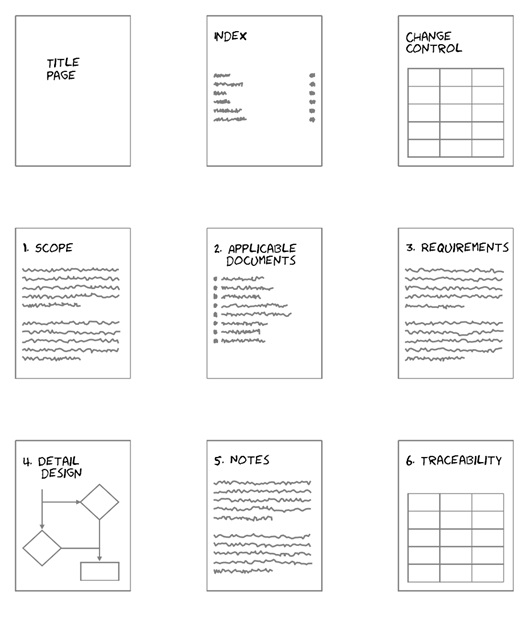
\includegraphics[width=0.7\linewidth]{./pictures/image1.jpg}
\caption{\label{fig:Agile}Agile development.}
\end{figure}
\end{center}

In the documentation, especially when talking about requirements and specifications, certain words convey additional meaning apart from their linguistic use. These words are usually capitalized.\\
\begin{itemize}
\item \textbf{SHALL} and \textbf{SHALL NOT} - Indicates a mandatory requirement.
\item \textbf{WILL} and \textbf{WILL NOT} - Indicates a declaration of purpose or an expression of simple futurity.
\item \textbf{SHOULD} and \textbf{SHOULD NOT} - Indicates a non-mandatory desire, preference or recommendation.
\item \textbf{MAY} and \textbf{MAY NOT} - Indicates a non-mandatory suggestion or permission.
\item \textbf{MUST} and \textbf{MUST NOT} should be avoided as it causes confusion with the above terms. 
\end{itemize}

\newpage

\section{System overview}
\subsection{Server Architecture}
%-----------------------Edit this section--------------------------
Linphone is a an IM application with VoIP capabilities based on the SIP (Session Initiation Protocol). The backbone of Linphone is the SIP server (Belle-SIP), we will be looking at the SIP architecture to analyse how it works and how group chat with encryption will be implemented in the Linphone application.\\
\\
SIP would not be able to function on a network without the use  of various devices and protocols. The essential devices are those that you and other participants would use in a conversation, allowing you to communicate with one another, and various servers may also be required to allow the participants to connect together. In addition to this, there are a number of protocols that carry your voice and other data between these computers and devices. Together, they make up the overall architecture of SIP.

\subsubsection{SIP Components}
There are two fundamental components that are used by the Session Initiation
Protocol:

\begin{itemize}
\item User agents,which are endpoints of a call or session (i.e.,each of the participants in a call or session).
\item SIP servers,which are computers on the network that service requests from clients,and send back responses.
\end{itemize}


\textbf{User Agent\\}
The mobile devices, laptops or computers that are being used to make the call and to receive the call or initiate sessions are known as user agents.\\
\\
User Agents can alternate as a UAC (User Agent Client) and UAS (User agent Server) depending on who initiated the session and who is responding; Because the user agent will send a message, and respond to another, it will alternate back and forth between these roles throughout a session. It will act as both the client and server.\\
\\

\textbf{SIP Server\\}
The SIP server is used to resolve usernames to IP addresses, so that requests sent from one user agent (mobile device)  to another can be directed properly. \\
\\
A user agent registers with the SIP server (currently each time the application is opened), providing it with their username and current IP address, thereby establishing their current location on the Linphone network. This also verifies that they are online, so that other user agents can see whether they’re available and invite them into a session, basically indicating the user agents presence. Because the user agent probably wouldn’t know the IP address of another user agent, a request is made to the SIP server to invite another user into a session.\\
\\
The SIP server then identifies whether the person is currently online, and if so, compares the username to their IP address to determine their location. \\
\\
In performing these various tasks of serving client requests, the SIP server
will act in any of several different roles:
\begin{itemize}
\item Registrar server
\item Proxy Server
\end{itemize}

\textbf{Registrar server\\}
Registrar servers are used to register the location of a user agent who has logged onto the Linphone network. Registrar servers play a huge role in providing location services to be used by the Proxy and Redirect servers. The location service is used to keep a database of those who have registered through Belle-SIP server,and where they are located.\\ 
\\
When a user agent registers with a Belle-SIP Registrar server, a REGISTER request is made. If the Registrar accepts the request, it will obtain the SIP address and IP address of the user agent, and add it to the location service for its domain.This database provides an up-to-date catalog of everyone who is online, and where they are located.

\begin{center}
\begin{figure}[H]
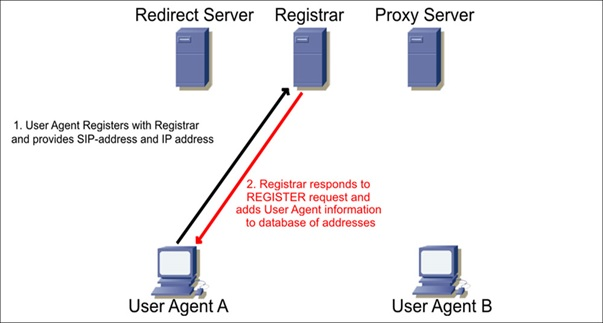
\includegraphics[width=1\linewidth]{./pictures/Registrar.JPG}
\caption{\label{fig:Registrar Server} Registrar Server}
\end{figure}
\end{center}

\textbf{Proxy Server\\}
It is a server that acts as an intermediary for request from clients seeking resources from servers.
A client (user agent) connects to the proxy server requesting some service, such as a file. Connection or other resource available from a different server and the proxy server server evaluates the request as a way to simplify and control its complexity.

\begin{center}
\begin{figure}[H]
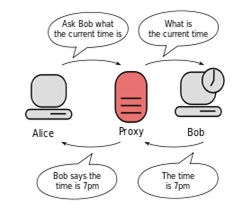
\includegraphics[width=0.7\linewidth]{./pictures/proxy1.JPG}
\caption{\label{fig:Proxy Server1} Proxy Server 1}
\end{figure}
\end{center}

\begin{center}
\begin{figure}[H]
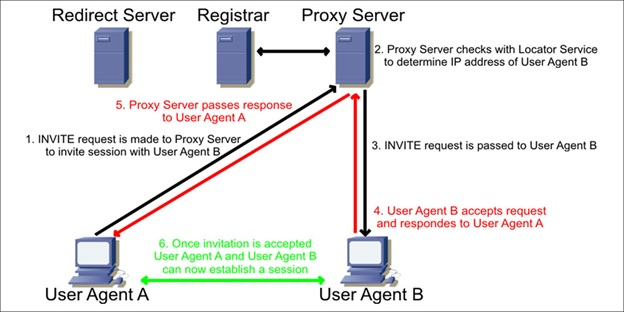
\includegraphics[width=1\linewidth]{./pictures/proxy2.JPG}
\caption{\label{fig:Proxy Server2} Proxy Server 2}
\end{figure}
\end{center}

\subsubsection{Client/Server and Peer-to-Peer(P2P) Architecture}
The Session Initiation Protocol uses two different types of architectures in network communications, both the:
\begin{itemize}
\item Client/Server Architecture
\item Peer-to-Peer (P2P) Architecture
\end{itemize}
\textbf{Client/Server Architecture}
\begin{itemize}
\item Client - requests specific services or resources
\item Server- dedicated to fulfilling requests by responding (or attempting to respond) with requested services or resources.
\end{itemize}

In VoIP, a client (mobile device) sends a request to register with a Registrar server, or makes a request to a Proxy Server or Redirect Server that allows it to connect with another user agent. In all these cases, the client’s role is to request services and resources, and the server’s role is to listen to the network and await requests that it can process or pass onto other servers.\\
\\
A server may run a number of services or have multiple server applications installed on it, a computer dedicated to the role of being a server may provide several functions on a network.
For example, a Web server might also act as an e-mail server. In the same way, SIP servers also may provide different services. A Registrar can register clients and also run the location service that allows clients and other servers to locate other users who have registered on the network. In this way, a single server may provide diverse functionality to a network that would otherwise be unavailable.

\begin{center}
\begin{figure}[H]
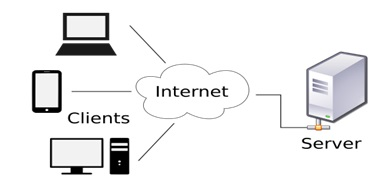
\includegraphics[width=1\linewidth]{./pictures/ClientServer.JPG}
\caption{\label{fig:Client/Server Architecture} Client/Server Architecture}
\end{figure}
\end{center}

\textbf{Peer-to-Peer Architecture\\}
Once the user agents have completed registering themselves, and making requests and receiving responses on the location of the user agent they wish to contact, the architecture changes from one of client/server to that of peer-to-peer (P2P). In a P2P architecture, user agents act as both clients who request resources, and servers that respond to those requests and provide resources. Because resources aren’t located on a single machine or a small group of machines acting as network servers, this type of network is also referred to as being decentralized.\\
\\
When user agents have initiated a session with one another, they become UAS (User Agent Clients) and UAS (User Agent Servers) to one another, and have the ability to invite additional participants into the session. Each of these User agents can communicate with one another in an audio or group chat. If one of these participants ends the session, or is using a device that fails during the communication, the other participants can continue as if nothing happened. This architecture makes communication between User agents stable, without having to worry about the network failing if one computer or device suddenly becomes unavailable.

\begin{center}
\begin{figure}[H]
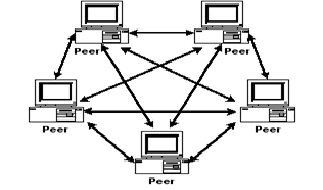
\includegraphics[width=1\linewidth]{./pictures/peer.JPG}
\caption{\label{fig:Peer-to-Peer Architecture} Peer-to-Peer Architecture}
\end{figure}
\end{center}

\subsubsection{Protocols used with SIP}
SIP works with different protocols at different stages of communication to pass data between servers, devices and participants. Without these protocols, communication would be impossible or insecure. A few protocols that will be used are User Datagram Protocol (UDP), Transport Layer Security (TLS).\\
\\
\textbf{User Datagram Protocol (UDP)\\}
UDP is used to transport units of data called datagrams over an IP network. UDP is faster than Transmission Control Protocol (TCP) because there is less processing of data. It is also used because when messages with small amounts of data are being sent across the network or when data will be unaffected by a few units of missing data.\\
\\
UDP shall be used in Linphones group chat implementation because it is fast for instant messaging and with Voice over IP when streaming a video, a minor loss of data will be a minor fault that generally would not affect the overall quality or performance. In this case, it is more important that data is passed quickly from one endpoint to another.\\
\\

\textbf{\large Transport Layer Security (TLS)\\}
TLS is used with other protocols like UDP to provide security between applications communicating over an IP network. TLS uses encryption to ensure privacy, so that third parties do not tamper with the messages being sent. A secure connection is established by authenticating the client and server or the User Agent Client and User Agent Server and then encrypting the connection between them. TLS is a multi-layered protocol that consists of a TLS Handshake Protocol and a TLS Record Protocol.\\
\\
The TLS Handshake protocol is used to authenticate the participants of the communication and negotiate an encryption algorithm. The client and server will have to agree upon an encryption method and prove who they are, using cryptographic keys before any data is sent between them. Once this has been done successfully, a secure channel is established between them. Once the TLS Handshake Protocol is used, the TLS Record Protocol ensures security that data is not modified and others cannot access the data while in transit.\\ 
\\
TLS may be used in Linphones implementation for a group chat to ensure that the messages are not modified and that it is securely transmitted to the other participants within the group chat therefore  the messages will be encrypted.\\
\\

\textbf{Session Description Protocol (SDP)\\}
SDP is used to send description information that is necessary when sending multimedia data across the network. It also provides information on what multimedia a user agent is requesting to be used and other information that is necessary in setting up the transfer of the data.\\
\\
SDP does not deliver media itself but is used between end points for negotiation of media type, format, and all associated properties. It contains the name and purpose of the session, the time the session is active, etc.\\
\\

\newpage

\section{Software overview}
\subsection{Software Architecture}

We will use LinphoneChatRoom interface to implement the group chat. LinphoneChatMessage will include createLinphoneChatMessage which will create a LinphoneChat. 
LinphoneCore : ge Core()  This will return a back pointer to the core managing the chat room.
LinphoneChatMessage.State
This class will show the state of an object. For example: Whether the file was transferred or not and whether the message was derived or not. It will keep track of certain actions that take place and track the progress.

%-----------------------Edit this section--------------------------
\newpage


\section{Certification considerations}
The project will be developed according to DO-178 certification requirements, for level D certification. Justification for level D is not dependant on safety considerations as is usually the case, but rather on limited time and the limited experience the team has with DO-178.\\
This project is not intended for avionics applications and is not safety critical, but rather serves as a case study on DO-178 software development.\\
\newpage

\section{Software lifecycle}
An agile software development methodology will be followed with this project:\\

\begin{center}
\begin{figure}[H]
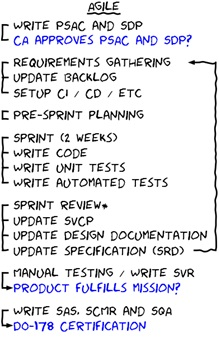
\includegraphics[width=0.5\linewidth]{./pictures/agile.jpg}\\
\caption{\label{fig:Agile}Agile development}
\end{figure}
\end{center}

%-------------------------

\subsection{Scrum}
During sprint planning and review sessions, we can review and update the Design Description (DD) document detailing the software architecture. At the end of a sprint, the implemented user stories will form the Software Requirements Data (SRD's). It will look something like this:

\begin{center}
\begin{figure}[H]
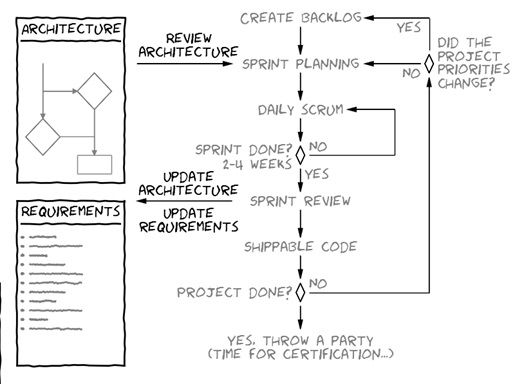
\includegraphics[width=0.7\linewidth]{./pictures/scrum.jpg}\\
\caption{\label{fig:Scrum}Scrum}
\end{figure}
\end{center}

During sprint planning we ensure that the user stories i.e. the high level requirements we are planning to implement is consistent with previous implemented requirements. During sprint review we update the requirements with the implemented user stories, and ensure the created functional tests and unit tests i.e. the low level requirements are consistent with the high level requirements (user stories).

%-------------------------

\subsection{Continuous integration (CI) and Continuous deployment (CD)}

The CI and CD servers themselves are effectively the Software Life Cycle Environment Configuration Index (SECI), Software Configuration Index (SCI) and parts of the Sofware Configuration Management Records (SCMR) deliverables. For this to be possible, the CI server must have a copy of the version control database when duplicated for certification. \\
This means an agile setup might look as follows:

\begin{center}
\begin{figure}[H]
\centering
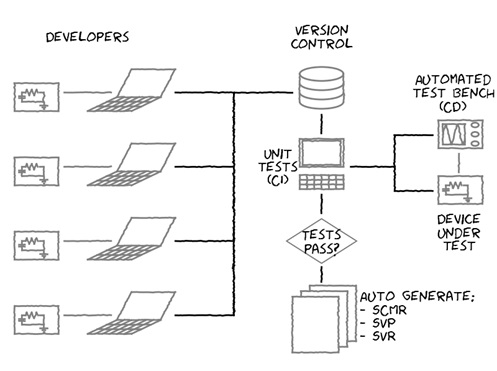
\includegraphics[width=0.7\linewidth]{./pictures/CI-CD.jpg}\\
\caption{\label{fig:CI/CD Output}CI and CD outputs}
\end{figure}
\end{center}

If all the tests pass, the CI / CD will autogenerate a snapshot of itself (VMs or some other duplication means) and the version control database to serve as the SECI and SCI. It will also generate reports of the tests run and their results to serve as the SVP and SVRs, and generate reports that can serve as SCMR items (This is baselines, commit histories etc.).


%-------------------------
\subsection{Test driven development}
Test driven development can be used to generate the large parts of the Software Verification Cases and Procedures (SVCPs) and Software Verification Results (SVRs). High level requirements will be developed and tested with feature driven development, and unit tests will be used to develop and test low level requirements. But not all unit tests are really low level requirements, for instance testing if a function can handle null pointer parameters. As such we will mark which unit tests are indeed low level requirements in the unit testing code itself.\\ 
\\
The relationship between the Continuous integration (CI) server and the Continuous deployment (CD) server is detailed in the popular test pyramid developed by Mike Cohn, where the CI is responsible for making sure the source code compiles at all times, and passes all unit tests, and the CD is responsible for making sure the automated functional tests pass at all times. One would expect to develop a lot more unit tests than functional tests, thereby limiting (but not eliminating) the need for expensive manual testing.\\
\newpage

%-------------------------

\section{Software development environment}

We will improve and revolve this sections out when we are comfortable in the project with the development environment.

\begin{itemize}
	\item Eclipse IDE
	\item Linux environment
	\item Java for user interface
	\item C for group chat functionality
	\item JUnit to test the Java code
	\item CUnit to test the C code
\end{itemize}
%\newpage

%-------------------------

\section{Software lifecycle data}

The following deliverables will be created during this project:

\begin{itemize}
	\item \textbf{Plan for Software Aspects of Certification (PSAC)}\\
		The Plan for Software Aspects of Certification is the primary means used by the certification authority for determining whether an applicant is proposing a software life cycle that is commensurate with the rigor required for the level of software being developed.
	\item \textbf{Software Development Plan (SDP)}\\
		The Software Development Plan includes the objectives, standards and software life cycle(s) to be used in the software development processes.
	\item \textbf{Software Verification Plan (SVP)}\\
		The Software Verification Plan is a description of the verification procedures to satisfy the software verification process objectives.
	\item \textbf{Software Requirements Data (SRD)}\\
		Software Requirements Data is a definition of the high-level requirements including the derived requirements.
	\item \textbf{Software Design Description (SDD)}\\
		The Design Description is a definition of the software architecture and the low-level requirements that will satisfy the software high-level requirements.
	\item \textbf{Source Code}\\
		This data consists of code written in source language(s) and the compiler instructions for generating the object code from the Source Code, and linking and loading data. This data should include the software identification, including the name and date of revision and/or version, as applicable.
	\item \textbf{Executable Object Code}\\
		The Executable Object Code consists of a form of Source Code that is directly usable by the central processing unit of the target computer and is, therefore, the software that is loaded into the hardware or system.
	\item \textbf{Software Verification Cases and Procedures (SVCP)}\\
		Software Verification Cases and Procedures detail how the software verification process activities are implemented.
	\item \textbf{Software Verification Results (SVR)}\\
		The Software Verification Results are produced by the software verification process activities.
	\item \textbf{Software Accomplishment Summary (SAS)}\\
		The Software Accomplishment Summary is the primary data item for showing compliance with the Plan for Software Aspects of Certification.
\end{itemize}
\newpage
%-------------------------

\section{Schedule / Software development plan}
The automated testing, setup of the CI and CD environment as well as the sprint back log will be implement and completed from the 22 June 2015 to the 5 July 2015 because that is when we conclude our exams and start implementations.
Please note that for each story we will setup unit testing and automated testing as discussed later on in the user role table.

\subsection{Task Description}
\begin{figure}[H]
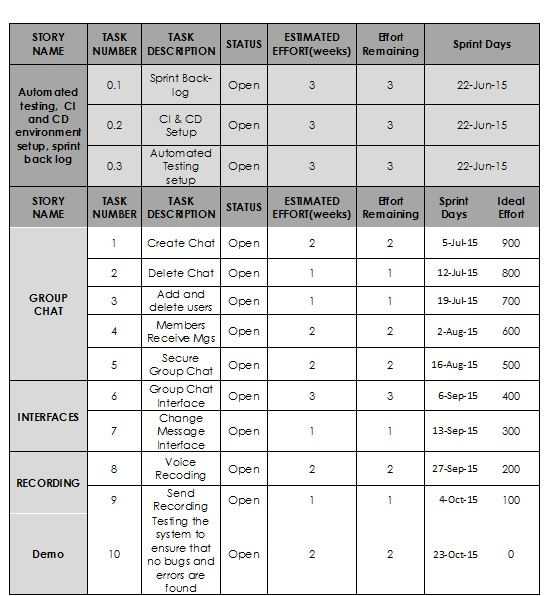
\includegraphics[width=1\linewidth]{./pictures/task.jpg}\\
\caption{\label{fig:Task Discription}Task Description}
\end{figure}

\subsection{User Roles}
Each task in the user story is implemented concurrently and sequentially as needed.

\begin{table}[h]
\centering
\caption{My caption}
\label{User Roles}
\begin{tabular}{ll}
Scrum master & Potego Mello\\
Client representative & Patience Mtsweni\\
UX developer & Lutfiyya Razak\\
Backend developer & Ephiphania Munava\\
Crypto developer & Tsepo Ntsaba and Lerato Molokomme\\
CI / CD support & Patience Mtsweni
\end{tabular}
\end{table}

\subsection{Burn Down Chart}
\begin{figure}[H]
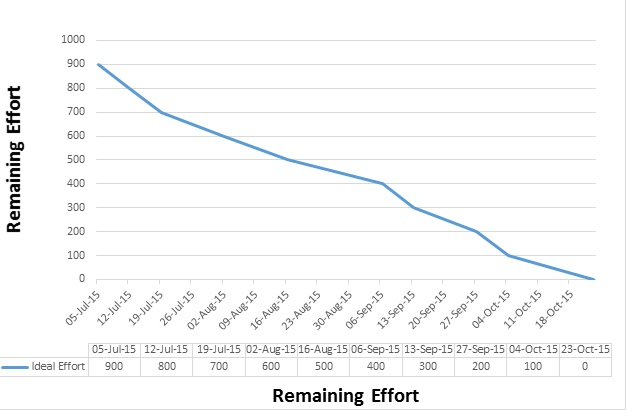
\includegraphics[width=1\linewidth]{./pictures/burnDown.jpg}\\
\caption{\label{fig:Burn-down chart}Burn-Down Chart}
\end{figure}
\newpage
%-------------------------

\section{Licencing and ownership}
The aim is to open-source the project which would be published on Github as forked from Linphone project. 
\end{document}
